\chptr{Proprietà dei Grafi Finiti}
\section{\underline{Relazione fondamentale dei grafi finiti}}
\begin{tcolorbox}[colback=yellow!30, colframe=yellow!30!black, title=Grafo finito]
Un grafo $G$ si dice finito se $V(G)$ è finito (numero finito di vertici).
\end{tcolorbox}

\begin{osservaz}
Un grafo finito ha un numero finito di lati:
$G$ finito $\Longrightarrow V(G)$ finito
$\Longrightarrow \binom{V(G)}{2} \text{ finito } \Longrightarrow E(G) \subseteq
\binom{V(G)}{2} \text{ finito } \Longrightarrow E(G) \text{ finito}$ (lemma dei cassetti).
Quindi $|E(G)|$ è finito.
\end{osservaz}

\begin{osservaz}
Esistono grafi infiniti che hanno numero finito di
lati: $(\mathbb{N}, \varnothing)$. Quindi avere lati finiti non implica la
condizione di essere grafo finito.
\end{osservaz}

\begin{tcolorbox}[colback=yellow!30, colframe=yellow!30!black, title=Grado di un vertice]
Sia $G=(V,E)$ un grafo finito e sia $v \in V$. Definitamo il grado di $v$
in $G$ come segue:
\[  \deg_G(v) := |\{e \in E| v \in e\}| \]
ovvero il numero di lati ai quali $v$ appartiene.
\end{tcolorbox}

\begin{tcolorbox}[colback=yellow!30, colframe=yellow!30!black, title=Score di un grafo]
Si chiama score di un grafo il vettore contenente il grado di ogni vertice,
eventualmente riordinati:
\[ \text{Score}(G) := (\deg_G(v_1),...,\deg_G(v_n)) = (d_1,...,d_n) \]
Lo score che ordina i gradi in modo crescente o al più costante è lo \textbf{score canonico}:
$d_1\leq ...\leq d_n$.
\end{tcolorbox}
Sottolineamo la relazione tra score di grafi isomorfi. Se $G$ e $G'$ sono isomorfi allora hanno lo stesso score:
\[ G \cong G' \Longrightarrow \text{Score}(G) = \text{Score}(G') \]
Non vale l'implicazione inversa.

\begin{tcolorbox}[title={Relazione fondamentale dei grafi finiti}]
Sia $G=(V,E)$ un grafo finito. Allora
\[ \sum_{v\in V} \deg_G(v) = 2|E| \]
\textit{\textbf{Dimostrazione:}} Scriviamo esplicitamente $V$ e $E$:
\[ V=\{v_1,...,v_n\} \qquad E=\{e_1,...,e_k\} \]
Dunque $n=|V|$ e $k=|E|$. Definiamo $m_{ij} \in \{0,1\}$ per ogni
$i \in \{1,...,n\}, j \in \{1,...,k\}$:
\[
    m_{ij} :=
    \begin{cases}
        0 & v_i \not \in e_j\\
        1 & v_i \in e_j
    \end{cases}
\]
Ottenendo la \textit{matrice di adiacenza}:
\[ 
    M =
    \begin{bmatrix}
        m_{11} & m_{12} & \dots  & m_{1k}\\
        m_{21} & m_{22} &        & \vdots\\
        \vdots &        & \ddots & \vdots\\
        m_{n1} & \dots  & \dots  & m_{nk}\\
    \end{bmatrix}
\]
Si osserva che la somma totale $\sum_{i=1}^{n}\sum_{j=1}^{k}m_{ij}$ degli elementi
della matrice non dipende dalla precedenza tra righe e colonne. Sommando
una riga si ottiene il grado del rispettivo vertice, mentre dalle
colonne si ottiene sempre 2, dal momento che ogni lato congiunge due
soli vertici:
\begin{align*}
    &\sum_{i=1}^{n}\left(\sum_{j=1}^{k}m_{ij}\right) = \sum_{j=1}^{k}\left(\sum_{i=1}^{n}m_{ij}\right)\Leftrightarrow\\
    &\Leftrightarrow \sum_{i=1}^{n}\deg_G(v_i) = \sum_{j=1}^{k}2\Leftrightarrow\\
    &\Leftrightarrow \sum_{v\in V}\deg_G(v)=2k=2|E|
\end{align*}
\cvd
\end{tcolorbox}

\begin{osservaz}
Una banale conseguenza della relazione fondamentale dei grafi finiti è
la semplicità con la quale si può calcolare $|E|$ (dato lo score $d$), cioè
il numero di lati del grafo $G$:
\[ |E| = \frac{1}{2}\sum_{v\in V}\deg_G(v) \]
\end{osservaz}

\section{\underline{Lemma delle strette di mano}}
Immaginiamo di essere ad una festa. Di norma ci si stringe spesso la
mano tra gli invitati, ma il padrone di casa si diverte a verificare
ogni volta una proprietà curiosa. Egli chiede sempre ad ogni ospite di
contare il numero di persone distinte con le quali ha stretto la mano.
Il padrone scopre sempre che il numero di invitati che hanno stretto la
mano ad un numero dispari di coetanei è \textit{sempre} pari. Da qui il
nome intuitivo del lemma delle strette di mano.
\begin{tcolorbox}[title={Lemma delle strette di mano}]
In un grafo finito il numero di vertici di grado dispari è pari.
$\\\\$
\textit{\textbf{Dimostrazione:}} Sia $G=(V,E)$. Definiamo:
\[ P:=\{v \in V| \deg_G(v) \text{ pari}\} \qquad D:=\{v\in V| \deg_G(v) \text{ dispari}\} \]
In particolare questi formano una partizione di $V$:
$V = P \cup D$ e $P \cap D = \varnothing$. Applicando
la relazione fondamentale otteniamo:
\[ \sum_{v\in P}\deg_G(v) + \sum_{v \in D}\deg_G(v) = 2|E| \Longleftrightarrow
\sum_{v\in D}\deg_G(v) = 2|E|-\sum_{v\in P}\deg_G(v) \]
Osserviamo che nel membro di destra abbiamo una quantità pari alla
quale si sottrae un'altra quantità pari. Questo implica che anche
il membro di sinistra è pari, ma essendo una somma di elementi dispari,
i suoi addendi devono comparire in numero pari.
\cvd
\end{tcolorbox}
Le applicazioni di questo lemma sono piuttosto vantaggiose in ambito
informatico. Supponiamo che, tra le specifiche di una rete che si
intende costruire, vengano forniti i numeri di collegamenti (cavi e
altro) per ogni dispositivo appartenente alla rete, sotto forma di score:
\[ s = (0,0,\textcolor{red}{1},\textcolor{red}{1},\textcolor{red}{1},2,2,\textcolor{red}{3},\textcolor{red}{3}) \]
Notiamo a colpo d'occhio che dovrebbero esistere 5 nodi di grado
dispari, ma questo non sarebbe possibile per il lemma delle strette
di mano.




\section{Grafi 2-connessi e hamiltoniani}
Sia $G=(V,E)$ un grafo con almeno due vertici. Scegliamo $v\in V$. Definiamo
il grafo $G - v$, ottenuto da $G$ cancellando il vertice $v$. Ponendo:
\[ V(G-v) := V(G) \setminus \{v\} \qquad E(G-v):= E(G)\setminus \{e\in E(G)| v \in e\} \]
Intuitivamente, $G-v$ è il grafo risultante dalla rimozione di un suo vertice
$v$ e della cancellazione dei lati ai quali esso appartiene.

\begin{tcolorbox}[colback=yellow!30, colframe=yellow!30!black, title=Grafo 2-connesso]
Sia $G=(V,E)$ con almeno 3 vertici. Diciamo che $G$ è 2-connesso se $G-v$ è
connesso $\forall v \in V$.
\end{tcolorbox}

Un grafo 2-connesso è semplicemente un grafo che, tolto un
qualsiasi vertice (uno soltanto), rimane sempre connesso.

Può essere desiderabile avere una rete di computer configurata
come un grafo 2-connesso. In tal modo, infatti, ammettendo che
i guasti e le manutenzioni affliggano sempre un solo nodo alla
volta, è garantita la connettività ai nodi rimanenti, senza che
un gruppo di essi rimanga isolato.

\begin{tcolorbox}[colback=yellow!30, colframe=yellow!30!black, title=Grafo Hamiltoniano]
Sia $G=(V,E)$ con almeno 3 vertici. Diciamo che $G$ è hamiltoniano se ammette
almeno un \textbf{ciclo hamiltoniano}, ovvero un ciclo in $G$ che attraversa
tutti i suoi vertici.
\end{tcolorbox}
\noindent Un grafo hamiltoniano è anche 2-connesso. Questo perché,
ammettendo un ciclo hamiltoniano, tale ciclo è di per se stesso
2-connesso.
Vale in generale la seguente catena di implicazioni (ma non quella inversa):
\[ G \text{ hamiltoniano } \Longrightarrow G \text{ 2-connesso } \Longrightarrow G \text{ connesso} \]
\begin{tcolorbox}[colback=yellow!30, colframe=yellow!30!black, title=Foglia]
Sia $G=(V,E)$ un grafo. Un vertice $v\in V$ si dice \textbf{foglia} di $G$
se $\deg_G(v)=1$.
\end{tcolorbox}
\noindent Supponiamo che $G=(V,E)$ sia 2-connesso. Allora $G$ non
può avere foglie. Infatti, si supponga per assurdo che $\exists v\in V$
foglia di $G$, cioè $\text{deg}_G(v)=1$. Allora $\exists!w\in V,w\not=v:\{v,w\}\in E$.
Considerando il grafo $G-w$, si osserva che $v$ è un vertice isolato di
$G-w$, dunque $G-w$ è sconnesso.
\begin{osservaz}
Lo stesso ragionamento vale per i grafi Hamiltoniani. Intuitivamente,
se $G$ fosse un grafo hamiltoniano, allora esisterebbe un ciclo hamiltoniano,
che cioè attraversa ogni vertice senza mai passare sugli stessi lati.
Ma allora non possono esistere foglie in $G$, altrimenti il ciclo
non potrebbe chiudersi (si potrebbe solo \emph{entrare}, ma non \emph{uscire}, dalla
foglia).
\end{osservaz}

\begin{figure}[H]
\centering
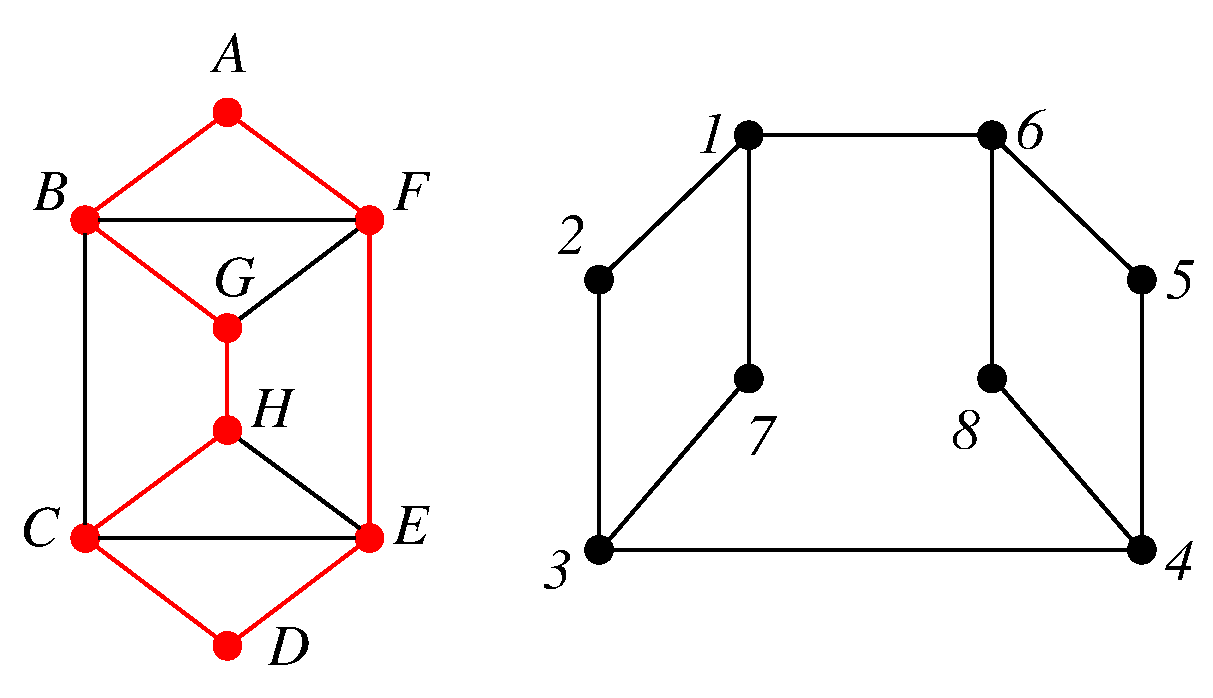
\includegraphics[scale = 0.4]{2-conn-vs-hamilton.pdf}
\caption{Un grafo hamiltoniano (a sinistra, con un ciclo evidenziato) e un grafo 2-connesso (a destra).
Si provi a verificare che quello a destra è effettivamente un grafo 2-connesso
cancellando un vertice qualsiasi (e i lati annessi)}
\end{figure}